\section{Information Obscurity}

Grundsätzlich ist anzunehmen dass jedes System irgendwann einer Attacke nachgibt. Das Information Obscurity Pattern stellt sicher, dass sensible Daten auch innerhalb des geschützten Systems bei einem möglichen ungewollten Zugriff weiter geschützt sind.

\begin{figure}[H]
	\centering
	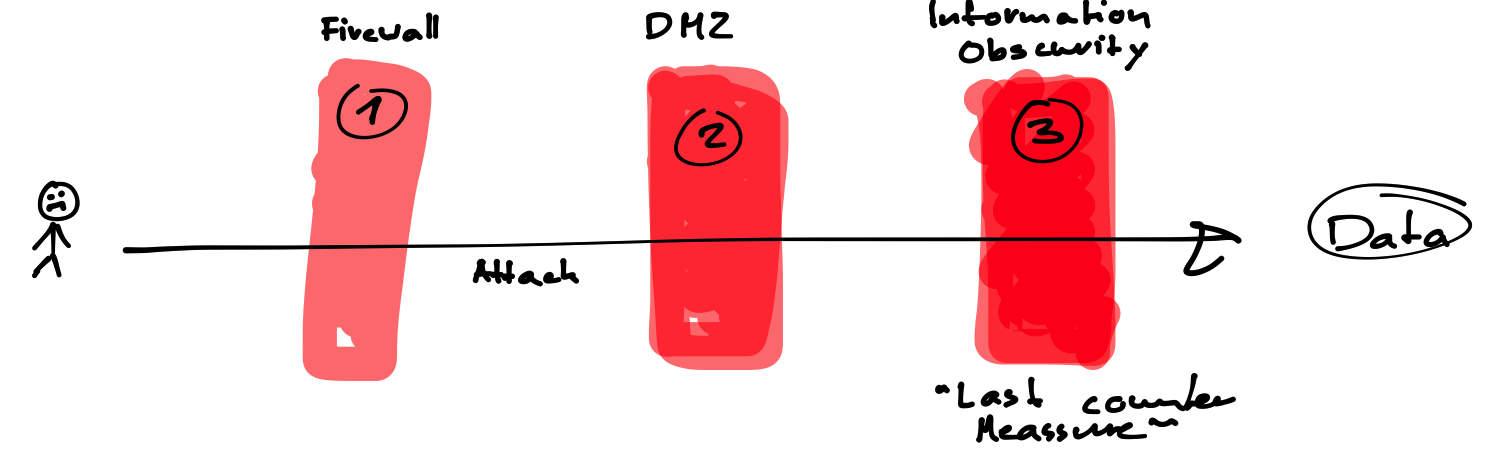
\includegraphics[width=12cm]{content/secure-internet-applications/images/information-obscurity-overview.png}
	\caption{Information Obscurity als letzte Sicherheitsmassnahme}
\end{figure}

\subsection*{Kontext}
Ein Internet Server-System (Webserver, Applikationsserver, Datenbankbackend etc.) tauscht zwischen den einzelnen Komponenten Informationen aus. Das System an sich ist bereits nach Aussen geschützt.

\subsection*{Problem}
Wie kann sichergestellt werden, dass sensitive Informationen welche zwischen den einzelnen Systemkomponenten ausgetauscht wird und evtl. innerhalb von diesen abgelegt ist beim Zugriff von Unbefugten weiterhin geschützt sind?

\begin{itemize}
	\item Es gilt abzuwägen welche Informationen überhaupt besonders geschützt werden sollen. Nicht jede Information ist hoch sensitiv und rechtfertigt die nötige Leistung zur Ver- und Entschlüsselung.
	\item Zu einer Ver- und Entschlüsselung sind entsprechende kryptographische Schlüssel notwendig. Diese gilt es wiederum entsprechend zu sichern.
\end{itemize}

\subsection*{Lösung}
Nachdem alle vorhandenen Informationsarten klassifiziert wurden, werden die als sensitiv bewerteten mittels passender Verschlüsselungsmechanismen zusätzlich gesichert.

Folgende Komponenten sind beim Information Obscurity Pattern beteiligt:

\begin{itemize}
	\item Ein \emph{Key} zur Ver- und Entschlüsselung der Informationen
	\item Ein \emph{Key Store} welcher die sichere Aufbewahrung und Herausgabe der Keys gewährleistet
	\item Eine \emph{Kryptographiekomponente} welche die eigentliche Arbeit übernimmt
\end{itemize}

Nicht zu vergessen ist natürlich die eigentliche Anwendungskomponente welche über die Kryptographiekomponente auf die verschlüsselten Informationen zugreift. Weiter sollte der Key Store über eine \emph{Protected Location} verfügen, in welcher er die Keys vor unbefugtem Zugriff geschützt (USB-Stick etc.)aufbewahren kann.

\subsection*{Ergänzungen}
\begin{itemize}
	\item Es ist nicht immer nötig, dass verschlüsselte Informationen entschlüsselt werden müssen, um auf deren Inhalt schliessen zu können.\\
	Beispiel: Passworthashes werden mit dem Hash der Benutzereingabe verglichen
	\item Jeder Schutz für sensitive Daten ist zwecklos, wenn bspw. der Webserver über einen Cache verfügt welcher alle gerenderten HTML-Informationen unverschlüsselt zwischenspeichert. Es gilt also jede Komponenten im System einem genauen Audit zu unterziehen.
	\item Der Sicherung von Konfigurationsinformationen (Keys) sollte besondere Aufmerksamkeit geschenkt werden: Oft können diese ohne es zu bemerken kopiert werden und somit die Information Obscurity Massnahmen nutzlos machen.
	\item Information Obscurity muss nicht zwingend mit einer Verschlüsselung im eigentlichen Sinne zusammenhängen: Bspw. kann man durch generische Bezeichnungen für Server (Sv1, Sv2 usw. statt Dataserver, Keyserver usw.) bereits dem potentiellen Eindringling bereits einen Stein in den Weg legen und dem eigenen Sicherheitsteam einen Zeitvorteil verschaffen.
	\item Wie so oft ist auch bei Information Obscurity die Balance zwischen Nutzen, Kosten und Performance zu finden.
\end{itemize}


\subsection*{Vorteile}
\begin{itemize}
	\item Sollte ein Angreifer in das gesicherte System gelangen, bietet Information Obscurity ein weitere Schicht an zusätzlicher Sicherheit für sensitive Informationen
	\item Da im optimalen Fall nicht alle Informationen mittels Information Obscurity geschützt werden, halten sich Performanceeinbussen in vertretbaren Grenzen.
\end{itemize}

\subsection*{Nachteile}
\begin{itemize}
	\item Die Performance kann tendenziell leiden wenn zu viele Informationen durch einen Ver- und Entschlüsselungsprozess geschleust werden müssen
	\item Die Komplexität des Systems erhöht sich, was wiederum Auswirkungen auf Wartbarkeit usw. hat.
	\item Komponenten welche von der Information Obscurity betroffen sind werden tendenziell aufwändiger und teurer in der Entwicklung.
\end{itemize}

\subsection*{Reallife Beispiele}
\begin{itemize}
	\item Verschiedenste OpenSource Projekte legen keine Klartext-Passwort in der Benutzerdatenbank ab sondern lediglich einen Hash (z.B. MD5) von diesem. Beim Login wird vom eingegebenen Passwort ebenfalls ein Hash erstellt und mit dem in der Datenbank hinterlegten verglichen.
	\item Beim Einbruch ins PlayStation Network von Sony (Online Gameing Platform für die Sony PlayStation Konsolen) wurden zig tausende Kreditkarteninformationen abgerufen und anschliessend auf dem Schwarzmarkt verkauft. Entsprechende Information Obscurity Massnahmen für eben diese Informationen hätten evtl. grösseren (Image-) Schaden eingrenzen können.
\end{itemize}

\subsection*{Mögliche Prüfungsfragen}
\begin{itemize}
	\item \emph{Welche Informationen sollten durch Information Obscurity geschützt werden?}\\
	Dies kann nicht generell beantwortet werden. Jedes System, jede Situation bedarf einer spezifischen Analyse und Klassifizierung der vorliegenden Informationen. Grundsätzlich sind aber für ein Unternehmen geschäftskritische Daten (seien diese operationeller oder aber auch rufbezogener Natur) tangiert.
\end{itemize}
